\newpage

\section{Results Part II: Case Study of Murrindindi Fire}\label{results_2}

\subsection{Historical Context}

In order to analyse the predictive power of our simulation, we perform a case study of the 2009 Australian Bushfires in the region of Murrindindi, Victoria. Our interest is to simulate the events known as the "Black Saturday bushfires" in the region and recreate the evolution of these fires using our cellular automaton model. Our aim is to quantify how well our simplified system predicts aspects of fire behaviour when working on the scale of tens of kilometers, and investigate if the real events differ from the predictions of our model.\newline
\indent Starting on February 7\textsuperscript{th}, 2009, a series of bushfires burnt over $450,000$ hectares of land and caused 173 fatalities in a series of events now referred to as the Black Saturday bushfires \cite{RoyalCommission}. The conditions at the time were ideal for a catastrophic wildfire event: Southeastern Australia had suffered from a prolonged period of low humidity and temperatures of over $45\degree$C. On Saturday 7\textsuperscript{th} at 14:55, a fire of unknown origin started in Northern Murrindindi, and it quickly spread across the landscape. Over the course of the day, the ensuing wildfire destroyed over 500 houses and resulted in the deaths of 39 people in the area of Marysville.
\subsection{Initial Conditions for Simulation}
\indent To simulate these events, geographical data including elevation and vegetation maps is obtained from the web portal for the Geoscience Department of the Australian Government \cite{Geodata}. A rectangular map spanning the coordinates  $(38.00 -37.00)$\degree S, $(145.50 - 147.00)$\degree E is used as an input for the simulation. The fire modelling array is overlaid on top of elevation data, and the simulation uses the vegetation map as its initial state. A colour-coded relief map is presented in Figure \ref{topography}, and the forest coverage of the same region is displayed in Figure \ref{forestcover}.

\begin{figure}[h!]
\centering
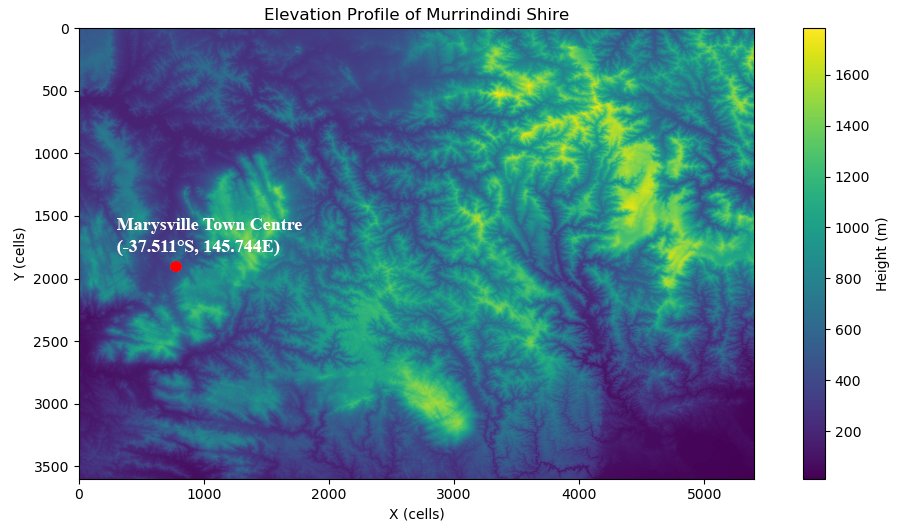
\includegraphics[width=0.83\textwidth]{Figures/elevation.png}\caption{Elevation data for Murrindindi Shire, $(38.00 -37.00)$\degree S, $(145.50 - 147.00)$\degree E}\label{topography}
\end{figure}

The relief map in Figure \ref{topography} shows substantial elevation changes in the region, where altitude changes from a minimum of $13$ metres to a maximum of $1783$ metres in less than $50$ kilometers on the ground. Wildfire has a tendency to travel uphill faster than downhill, and we expect our model to simulate this effect in the regions where the local surface gradient is the most pronounced. The data for elevation is used to calculate the fire propagation coefficients as described in Section \ref{factors}.\newline
\indent For the vegetation data, we use a topographical map with forest coverage data, accessed through Geoscience Australia's Web Portal \cite{Geodata}. We binarize the landscape into two possible values: cells with forest cover are assigned a value of $0$ (fuel), and cells without forest are assigned a value of $1$ (non-flammable). The output is shown in Figure \ref{forestcover}.

\begin{figure}[h!]
\centering
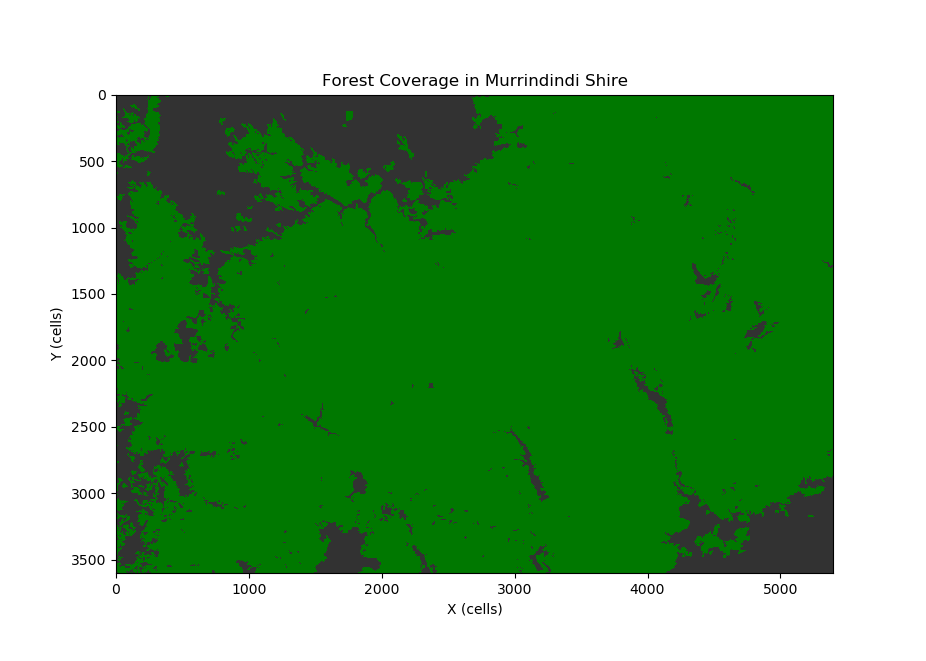
\includegraphics[width=0.9\textwidth]{Figures/ForestCover.png}\caption{Map of forest coverage in Murrindindi Shire. Woodland is represented by green and non-flammable terrain (including water) is shown in gray.}\label{forestcover}
\end{figure}

\noindent To analyse our model in the simulated real-world scenario of the Murrindindi fires, we perform a simulation of duration $N=500$ time steps, with different sets of environmental variables on each run. The cell arrays for elevation and vegetation were resized to dimensions $(540 \times 360)$ to maintain a feasible run time. The fire duration $\Delta t$ was configured to $2$ time steps, and the strength parameters $\alpha$ and $\beta$ and spotting parameters $E,M$ and $\sigma$ are varied across different runs. The results are shown in Figures \ref{fig:vegeOnly} to \ref{fig:allParams}, and we compare these to the real observations of the bushfires, shown in Figure \ref{fig:realData}.

\subsection{Fire Simulation Results}
\begin{figure}[H]
  \centering
  \begin{subfigure}[t]{0.47\textwidth}
    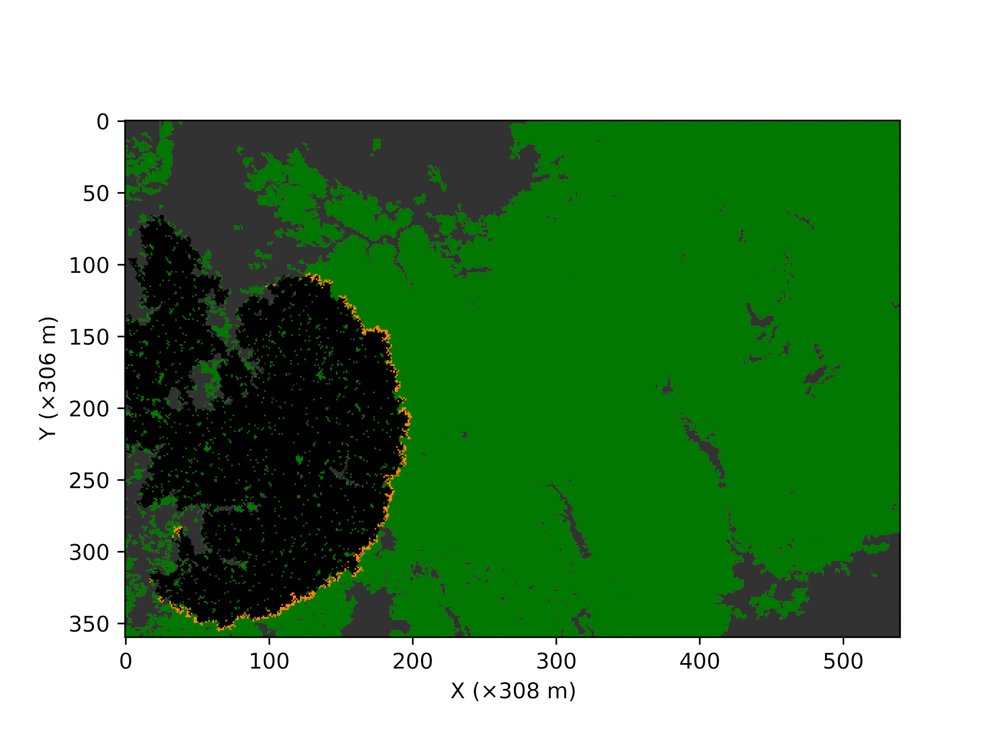
\includegraphics[width=0.95\textwidth]{Figures/LastFrame_01.jpg}
    \caption{Simulation run with vegetation data only, \,\, iterated for a duration of $500$ time steps}
    \label{fig:vegeOnly}
  \end{subfigure}
  %
  \begin{subfigure}[t]{0.47\textwidth}
    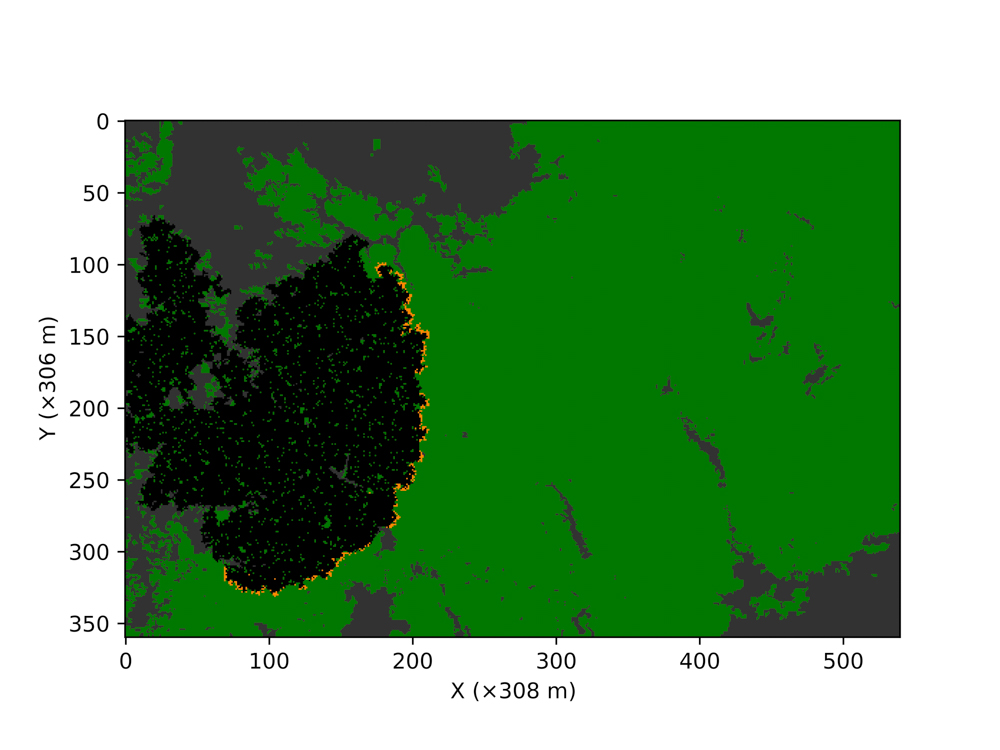
\includegraphics[width=0.95\textwidth]{Figures/LastFrame_02.jpg}
    \caption{Simulation with vegetation and elevation data, $\alpha=0.045, \beta = 0$, iterated $500$ time steps}
    \label{fig:vegePlusEle}
  \end{subfigure}
  %
  \begin{subfigure}[t]{0.47\textwidth}
    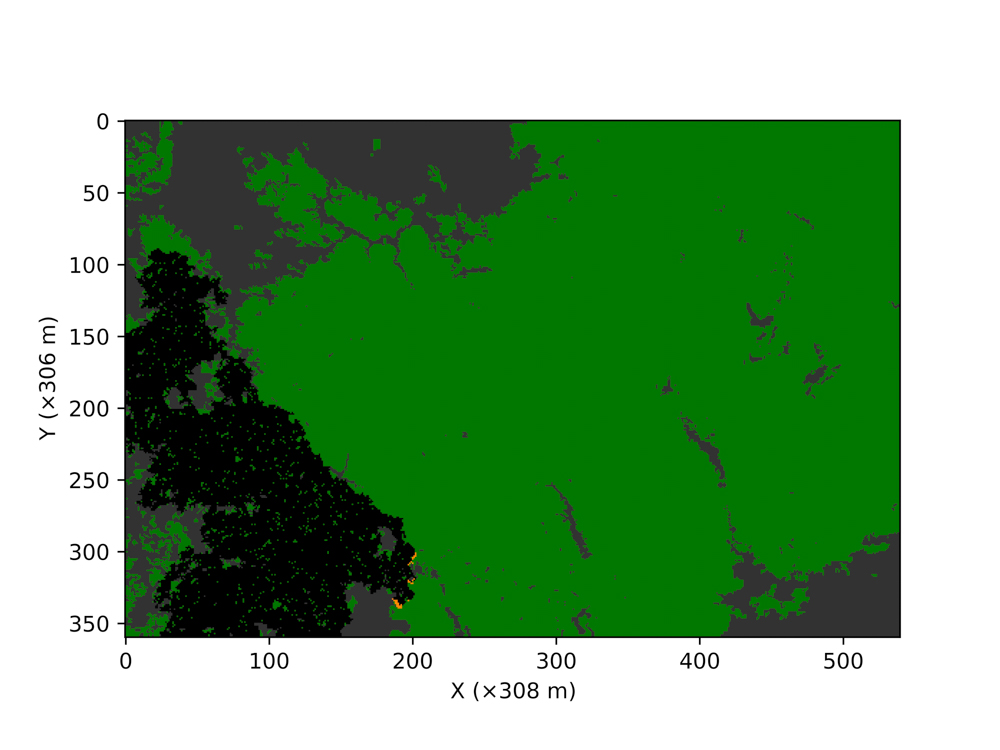
\includegraphics[width=0.95\textwidth]{Figures/LastFrame_03.jpg}
    \caption{Simulation with vegetation and wind data, $\alpha=0, \beta = 0.1$, iterated $500$ time steps}
    \label{fig:vegePlusWind}
  \end{subfigure}
  %
  \begin{subfigure}[t]{0.47\textwidth}
    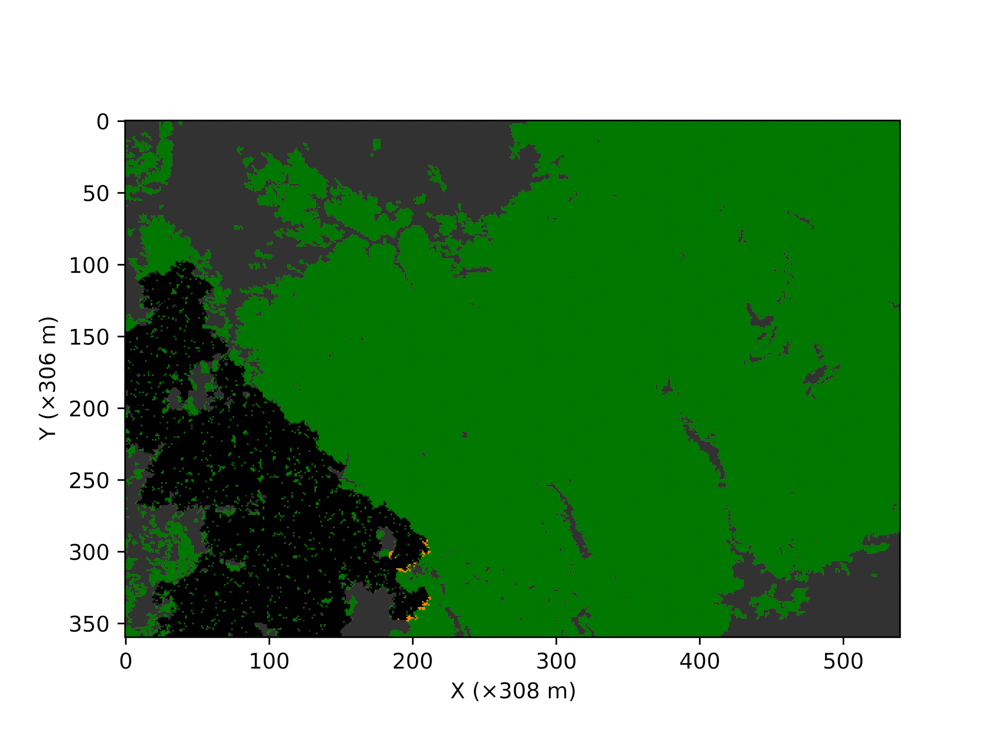
\includegraphics[width=0.95\textwidth]{Figures/LastFrame_04.jpg}
    \caption{Simulation with vegetation, elevation and wind data, $\alpha=0.045, \beta = 0.1$, $500$ time steps}
    \label{fig:vegePlusElePlusWind}
  \end{subfigure}
  %
  \begin{subfigure}[t]{0.47\textwidth}
    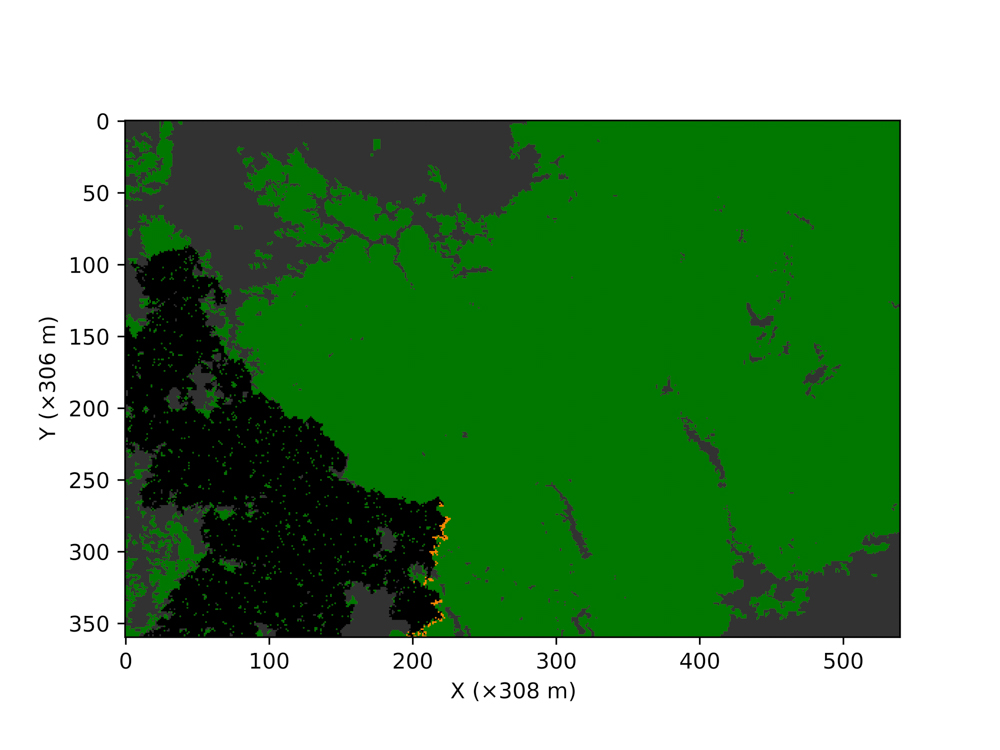
\includegraphics[width=0.95\textwidth]{Figures/LastFrame_05.jpg}
    \caption{Simulation with vegetation, wind and ember data, $\alpha=0, \beta = 0.1$, iterated $500$ time steps}
    \label{fig:almostAllParams}
   \end{subfigure}
   %
   \begin{subfigure}[t]{0.47\textwidth}
    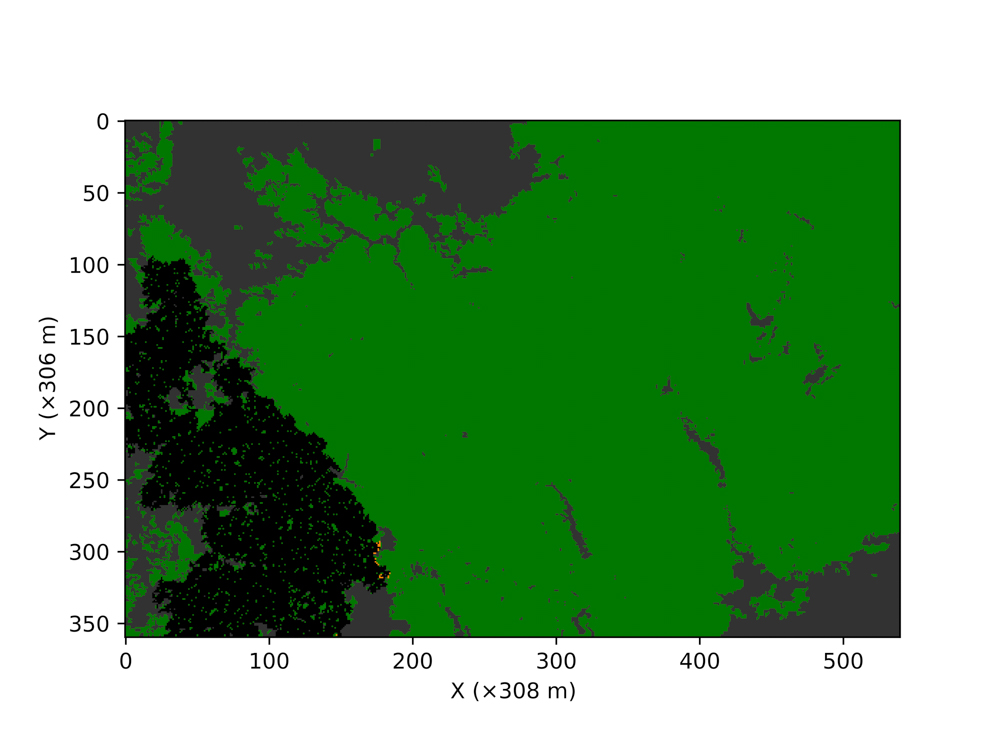
\includegraphics[width=0.95\textwidth]{Figures/LastFrame_06.jpg}
    \caption{Simulation with vegetation, elevation, wind and ember data, $\alpha=0.045, \beta = 0.1$, $500$ steps}
    \label{fig:allParams}
   \end{subfigure}
   \caption{End result of Murrindindi fire simulation after 500 time steps.  Colour code: \newline green = fuel cells, orange = fire cells, black = burnt cells, grey = non-fuel cells.}
\end{figure}

\noindent In Figure \ref{fig:vegeOnly}, we observe that the fire front is uniform in the flammable area, and approximately symmetrical around its centre. This demonstrates that in the absence of other factors, fire will propagate evenly in all directions where fuel is present. In Figure \ref{fig:vegePlusEle}, the added elevation data breaks the symmetry of the fire front, and fires have preferential directions based on the surface gradient.\newline \indent
For the simulation using wind data, we configured the wind velocity to $52$ km/h South-South-Easterly, as measured at the local Coldstream Automatic Weather Station at 18:00 \cite{RoyalCommission}. The effect of wind is seen in Figure \ref{fig:vegePlusWind}, where the fire front propagates uniformly along the direction of the wind, with only minor deviations from the path. When the effects of elevation and wind are combined, we observe that wind largely dictates the direction of the fire, as seen in Figure \ref{fig:vegePlusElePlusWind}. Here, the resulting path of fire is almost identical to that traced out in Figure \ref{fig:vegePlusWind} where wind is the only additional factor. \newline \indent
To test the effect of spotting on the path of fire, we configured each burning cell to send out $E=10$ embers, which remain on fire for a duration of $t_f = 30$ seconds. A fuel cell was set to ignite on average by $M=50$ embers, with a standard deviation of $\sigma=10$. The result of a simulation incorporating wind and ember data is shown in Figure \ref{fig:almostAllParams}. We observe that the effect of spotting speeds up the rate of fire spread along the direction of the wind, visible at the bottom of the map where the fire front has advanced further South than it did in the simulation with wind data alone.\newline \indent
For the final test, we ran the simulation using all available parameters: elevation, wind and spotting. The result after $500$ time steps is displayed in Figure \ref{fig:allParams}. We remark that the end result is comparable to previous results with wind data, with a small difference in the lower section of the map where the change in elevation at the bottom of the map inhibited the fire from propagating to certain downhill areas.

\subsection{Comparison to Real Events}
To assess the accuracy of the model, we compare its results to the actual events of the Murrindindi fires, as captured by satellite images. In totality, the Murrindindi fire burnt an area of $43,154$ hectares over the course of $27$ days. We analyse the differences between our model and real-world events by calculating the total surface area burnt in the fire simulation, and compare these values to the actual area burnt by the real fires. Due to a long run time of $\sim 7$ hours for each simulation, the data obtained is a direct non-averaged output generated in a single instance. The results are presented in Table \ref{Tab:areaburnt}. \newline
\indent We observe that our model significantly overestimates in the amount of area burnt when compared to the physical events, and our results differ from the target of $43,154$ hectares by up to two orders of magnitude (Figure \ref{fig:vegeOnly}). Based on the area burnt, the most accurate versions of the model include the effects of wind (Figures \ref{fig:vegePlusWind} - \ref{fig:allParams}). This suggests that wind is a primary factor in determining the accuracy of a wildfire simulation.

\newpage

\begin{table}[h!]
    \centering
    \begin{tabular}{|c|c|}
    \hline
     \textbf{Figure} & \textbf{Area burnt} (ha)\\ \hline
     \ref{fig:vegeOnly} & $1,137,690$ \\ \hline
     \ref{fig:vegePlusEle} & $1,039,539$ \\ \hline
     \ref{fig:vegePlusWind} & $254,428$\\ \hline
     \ref{fig:vegePlusElePlusWind} & $389,184$\\ \hline
     \ref{fig:almostAllParams} & $370,444$\\ \hline
     \ref{fig:allParams} & $425,608$\\ \hline
     \ref{fig:realData} (target) & $\mathbf{43,154}$\\ \hline
    \end{tabular}
    \caption{Total surface area burnt in wildfires as $t\xrightarrow{}\infty$}\label{Tab:areaburnt}
\end{table}

\noindent In the case of Figures \ref{fig:vegeOnly} and \ref{fig:vegePlusEle}, the surface area burnt in the simulation is approximately $90\%$ of the total area of flammable material. This is in contrast to the real events, where the fires remained localised in the Marysville area and were confined  within a $\sim 25$km radius of the town centre. An infrared image of Marysville and its surroundings on February 16\textsuperscript{th}, 2009 is provided for reference in Figure \ref{fig:realData}:

\begin{figure}[h!]
    \centering
    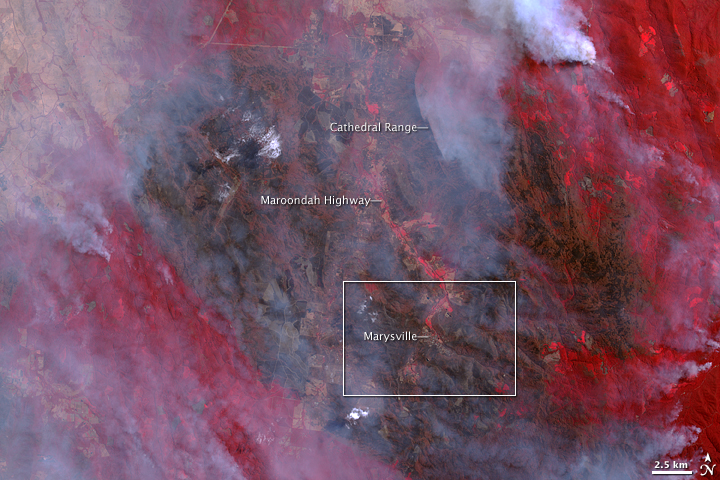
\includegraphics[width=0.9\textwidth]{Figures/realFire.jpg}
    \caption{Murrindindi fires (infrared image), 16/02/2009, NASA Earth Observatory \cite{NASA}}
    \label{fig:realData}
\end{figure}

\noindent We note that the above results vary substantially for different values of the strength parameters $\alpha$ and $\beta$. Previous work has determined that a value of less than $0.1$ for both $\alpha$ and $\beta$ shows the most accurate behaviour \cite{Aleksandridis_2008}, however the exact values need be determined via non-linear fitting methods such as Nelder-Mead optimization \cite{Denham_2018}. As determined in Section \ref{modellimits}, there are parameter-specific limits at which the fire behaviour becomes non-physical. To avoid this we selected the values $\alpha = 0.045$ and $\beta = 0.1$ for elevation and wind respectively. \newline
\noindent For the parameters related to embers, our method is novel to the literature. As such, there was no previous analysis on the ideal number of embers emitted by fire, and we determined the values $E=10, M=50$, $t_f = 30s$ and $\sigma=10$ based on trial and error.\newline \indent
We postulate that the main reason behind the discrepancy between our model and the real-world events is the static nature of the environmental conditions in our model. Firstly, the wind speed and direction is a fixed variable in our model, whereas in the real world there were major changes in wind direction occurring on February 7\textsuperscript{th}. Secondly, the real bushfires burnt out as a result of a change in weather conditions and continued human efforts, whereas our model lacks these stabilising factors. Thirdly, our cellular automaton is defined using a binary criterion where a cell is either flammable or not, so it does not fully represent different types of possible fuel. In a real environment, a bushfire has a different ignition probability than a canopy or a grass fire, and the fire duration varies across different vegetation types. \newline\indent
We theorise that the lack of moderating factors in our model causes the simulated fires to spread out until most of the fuel source is burnt, especially in the models without wind effects. An example of this is shown in Figure \ref{fig:endFrame}, where we show the state of a Murrindindi simulation with $\Delta t=2$ after $1000$ time steps using vegetation data.

\begin{figure}[h!]
    \centering
    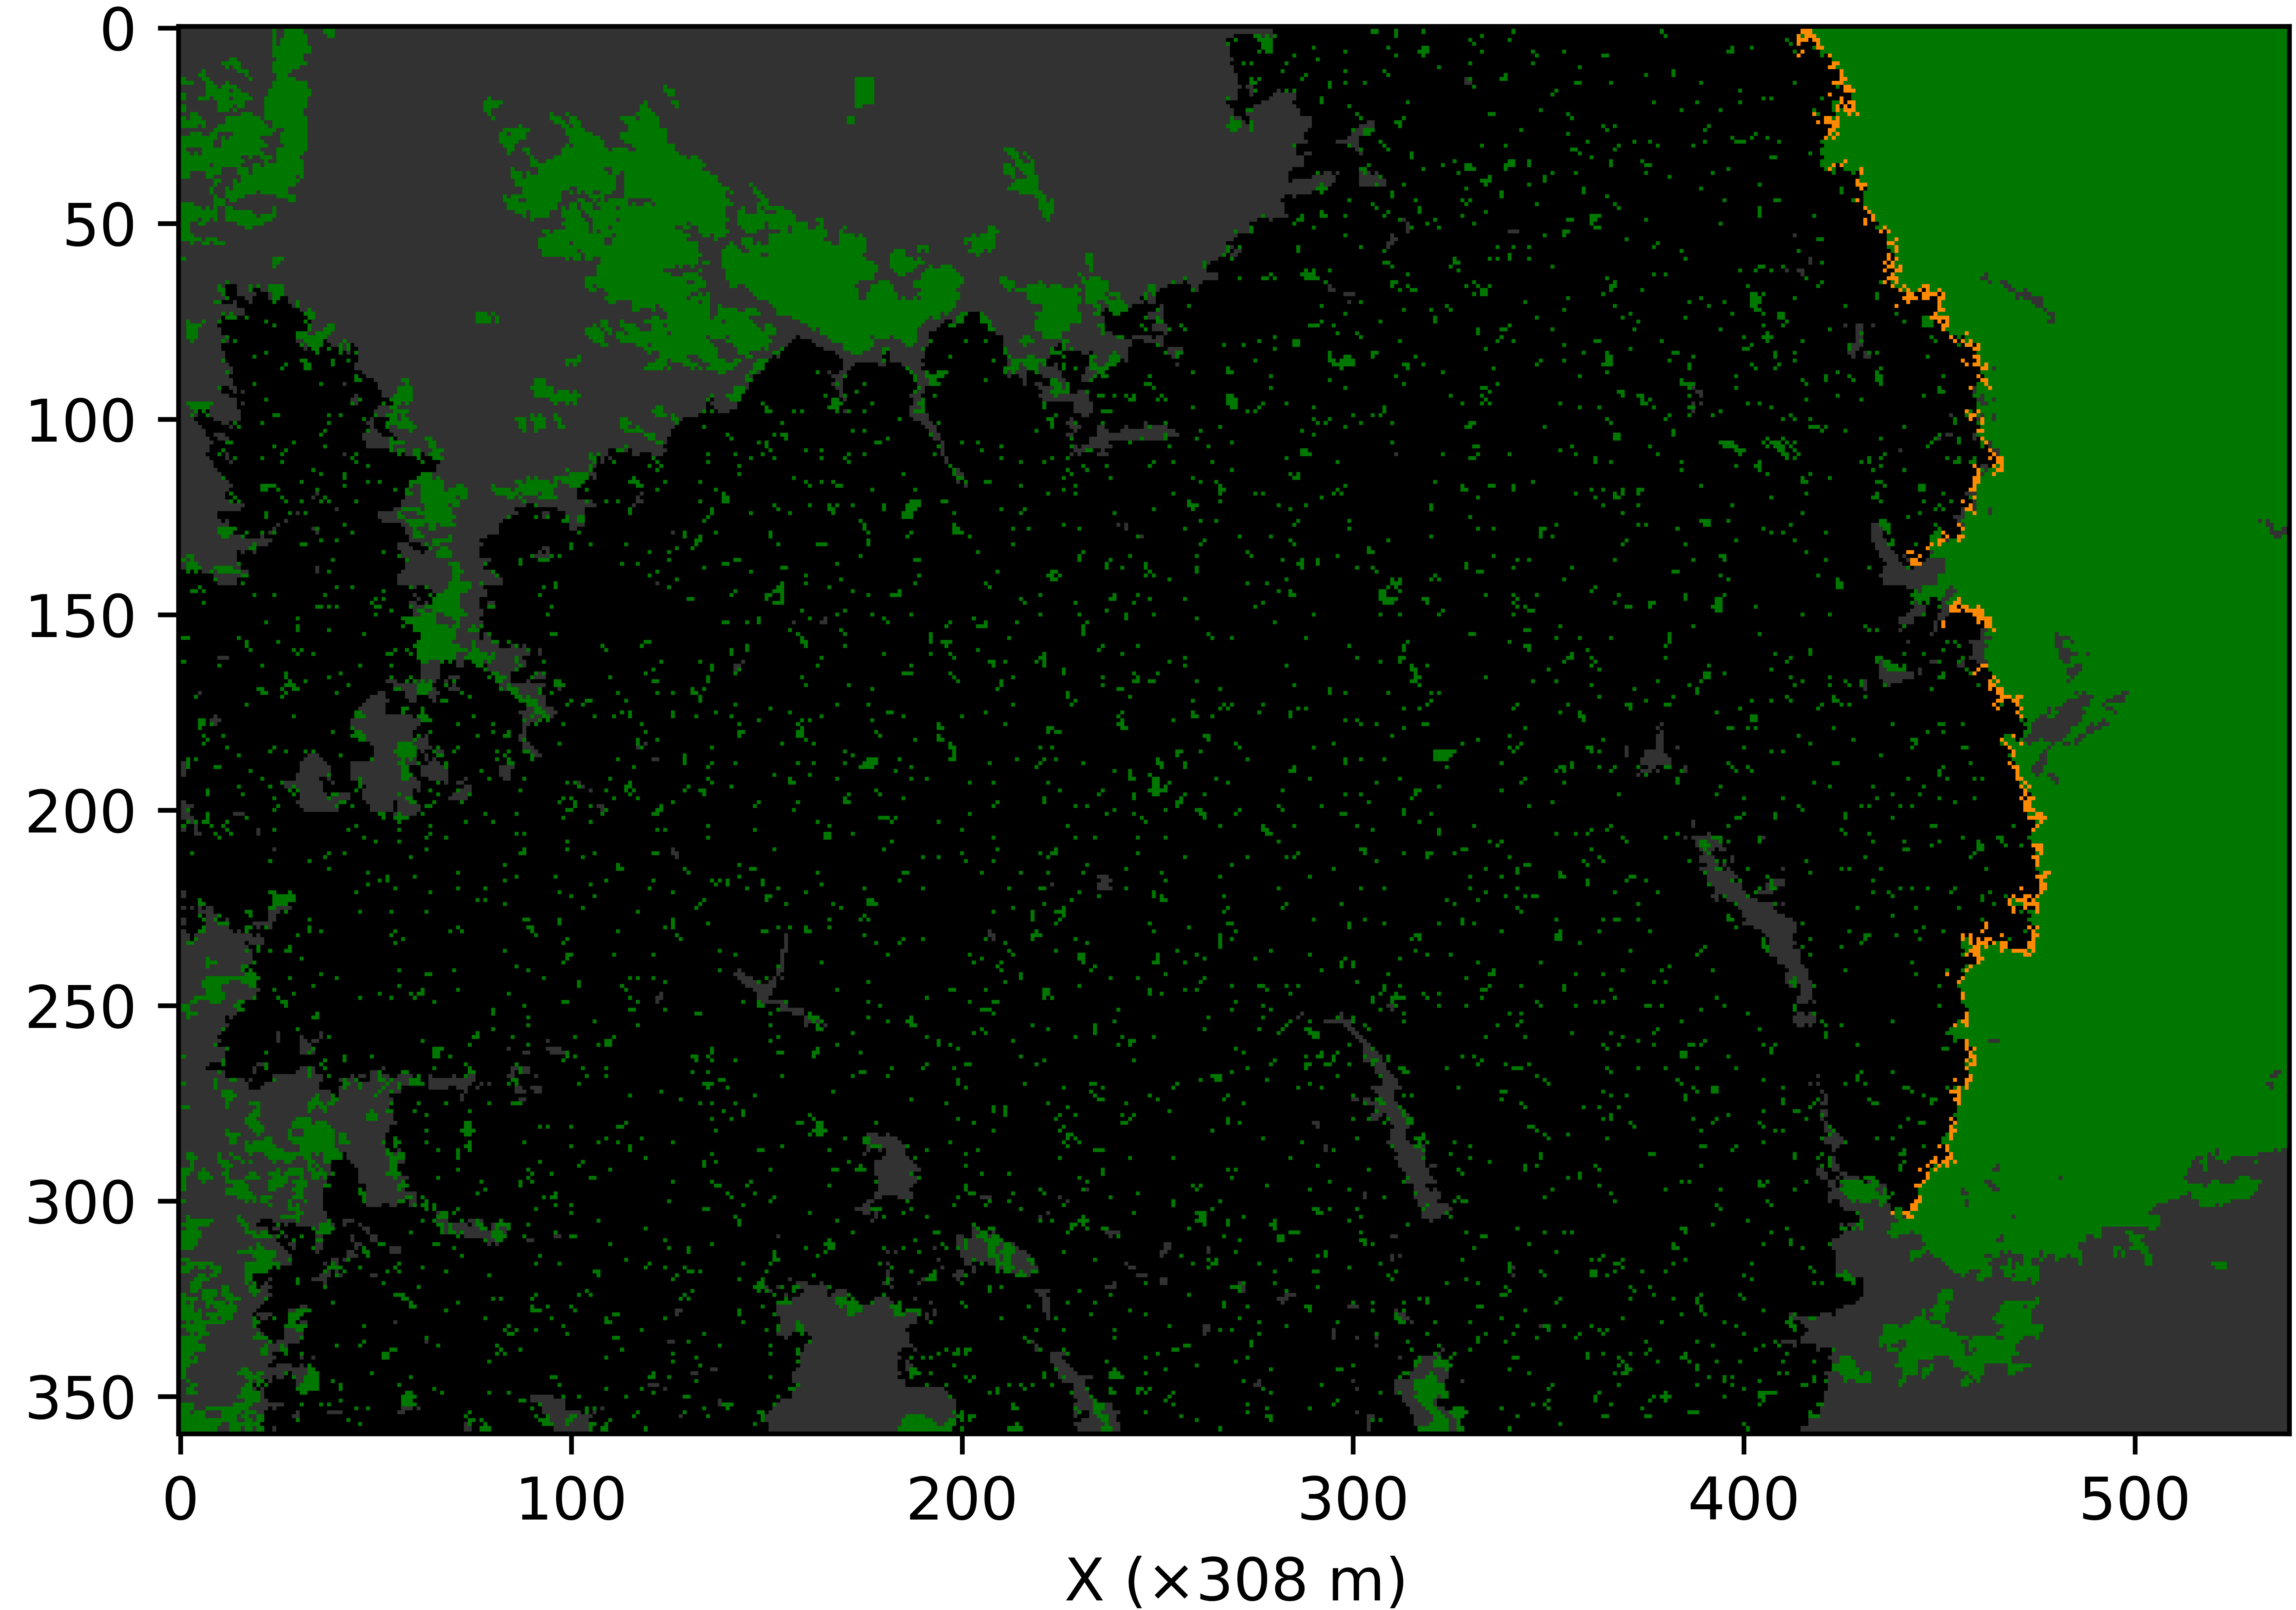
\includegraphics[width=0.5\textwidth]{Figures/LastFrame.png}
    \caption{End result of fire simulation, duration 1000 time steps.}
    \label{fig:endFrame}
\end{figure}

\indent We observe that in the absence of wind, the fire spreads unconstrained across the whole landscape, burning over $90\%$ of the fuel source. This is an unrealistic result, as real wildfires tend to extinguish over time due to changes in weather conditions. To overcome this limitation in our current simulation, a more accurate model must reflect possible environmental changes in the net fuel ignition probability. Further work is also required to determine the control parameters $\alpha,\beta,E,M,t_f$ and $\sigma$ to balance the effect of elevation, wind and spotting. To this end, we suggest improvements to the model in Section \ref{furtherwork}.